\documentclass[10pt, aspectratio=169]{beamer}

% ==========================================
% Theme & Color Settings (Moloch Theme)
% ==========================================
\usetheme{moloch}
\usecolortheme{moloch}

% ==========================================
% Modular Preambles & Configurations (Relative)
% ==========================================
\input{../../preamble/packages.tex}
\input{../../preamble/macros.tex}
\input{../../preamble/listings-setup.tex}

% ==========================================
% Presentation Metadata
% ==========================================
\title{Heterogeneity-Aware Adaptive Federated Distillation for Smart Campus Energy Management}
\subtitle{Research Progress Update}
\author{Christian Joseph Bunyi \\ \small Advisor: Fritz Flores}
\institute{Dr. Andrew L. Tan Data Science Institute \\ De La Salle University}
\date{\today}

% ==========================================
% Slide Deck Document Structure
% ==========================================
\begin{document}

% Slide 1: Title Slide
\begin{frame}[plain]
    \titlepage
\end{frame}

% ==========================================
% Topic 1: Edge ML & Smart City/Campus
% ==========================================

% Slide 2: Challenge-oriented taxonomy
\begin{frame}{Edge ML \& Smart City/Campus}
    \centering
    \vfill
    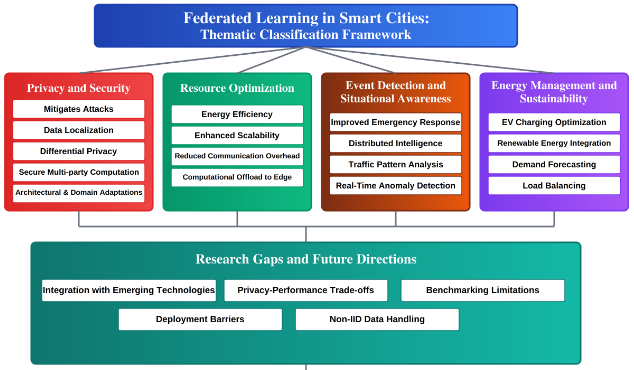
\includegraphics[width=\textwidth,height=0.7\textheight,keepaspectratio]{figures/alterkawi_fig2.png}
    \vspace{0.15cm}

    {\fontsize{5.5pt}{7pt}\selectfont Alterkawi and Dib (2025), Figure 2: Challenge-oriented taxonomy of FL applications in smart cities.\\}
    \vspace{0.05cm}
    {\fontsize{8pt}{9.5pt}\selectfont Energy management and resource optimization are primary FL challenges in urban environments.}
    \vfill
\end{frame}

% Slide 3: Smart city data sources
\begin{frame}{Edge ML \& Smart City/Campus}
    \centering
    \vfill
    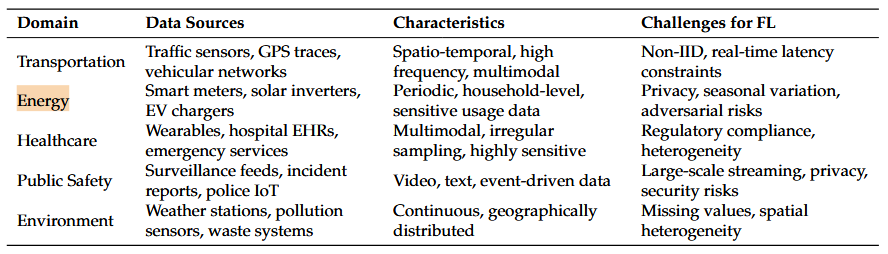
\includegraphics[width=\textwidth,height=0.7\textheight,keepaspectratio]{figures/alterkawi_table2.png}
    \vspace{0.15cm}

    {\fontsize{5.5pt}{7pt}\selectfont Alterkawi and Dib (2025), Table 2: Representative smart city data sources and characteristics.\\}
    \vspace{0.05cm}
    {\fontsize{8pt}{9.5pt}\selectfont Urban energy and environmental data are multimodal, continuous, and heterogeneous.}
    \vfill
\end{frame}

% Slide 4: Future research areas
\begin{frame}{Edge ML \& Smart City/Campus}
    \centering
    \vfill
    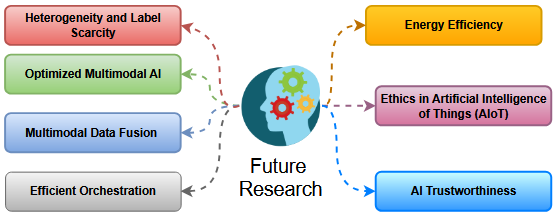
\includegraphics[width=\textwidth,height=0.7\textheight,keepaspectratio]{figures/cajas_fig8.png}
    \vspace{0.15cm}

    {\fontsize{5.5pt}{7pt}\selectfont Cajas Ordóñez et al. (2025), Figure 8: Future research areas for machine learning at the edge.\\}
    \vspace{0.05cm}
    {\fontsize{8pt}{9.5pt}\selectfont Data heterogeneity, energy efficiency, and orchestration are the main bottlenecks for Edge ML.}
    \vfill
\end{frame}

% ==========================================
% Topic 2: Smart Campus Energy Management
% ==========================================

% Slide 5: Theoretical energy savings
\begin{frame}{Smart Campus Energy Management}
    \centering
    \vfill
    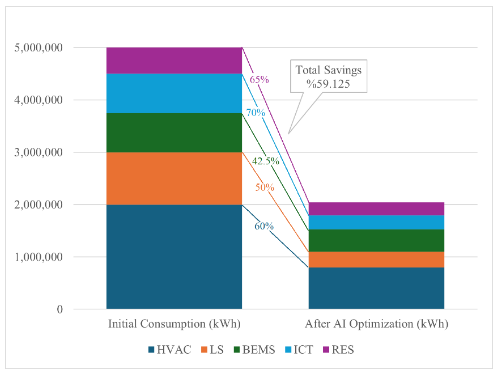
\includegraphics[width=\textwidth,height=0.7\textheight,keepaspectratio]{figures/manassra_fig8.png}
    \vspace{0.15cm}

    {\fontsize{5.5pt}{7pt}\selectfont Manassra and Işık (2025), Figure 8: Theoretical energy savings in a mid-sized smart campus.\\}
    \vspace{0.05cm}
    {\fontsize{8pt}{9.5pt}\selectfont AI optimization can achieve up to 60\% energy savings for campus HVAC systems.}
    \vfill
\end{frame}

% Slide 6: AI technologies in smart campus
\begin{frame}{Smart Campus Energy Management}
    \centering
    \vfill
    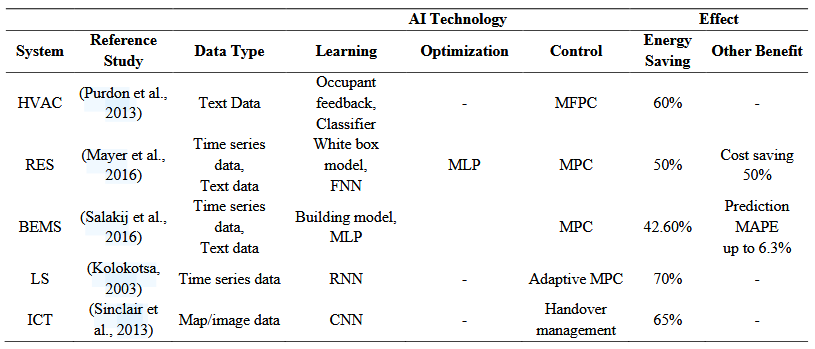
\includegraphics[width=\textwidth,height=0.7\textheight,keepaspectratio]{figures/manassra_table2.png}
    \vspace{0.15cm}

    {\fontsize{5.5pt}{7pt}\selectfont Manassra and Işık (2025), Table 2: Artificial intelligence technologies in smart campus systems.\\}
    \vspace{0.05cm}
    {\fontsize{8pt}{9.5pt}\selectfont Different ML models (such as MLPs, CNNs, and RNNs) target specific campus subsystems.}
    \vfill
\end{frame}

% ==========================================
% Topic 3: Non-IID Quantification & Compression
% ==========================================

% Slide 7: Non-IID Skew/Distribution
\begin{frame}{Non-IID Quantification \& Compression}
    \centering
    \vfill
    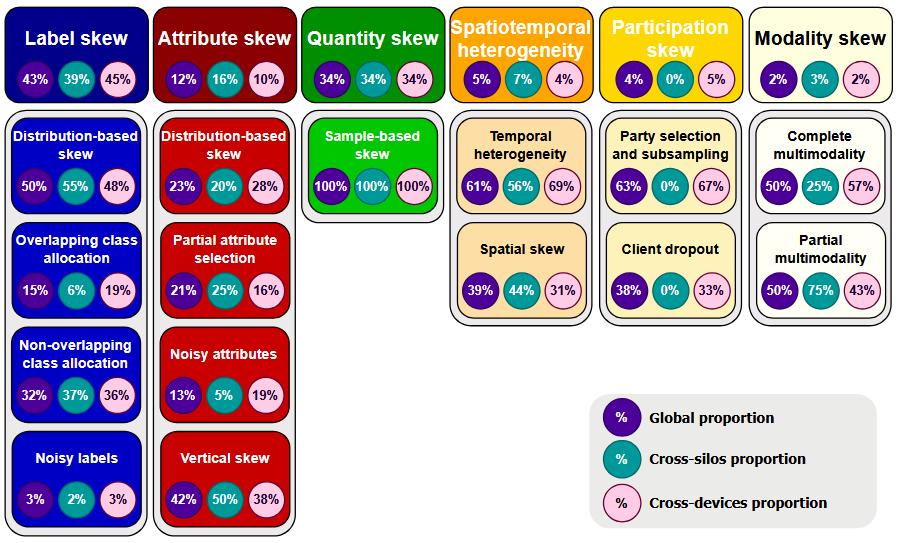
\includegraphics[width=\textwidth,height=0.7\textheight,keepaspectratio]{figures/jimenez_fig7.png}
    \vspace{0.15cm}

    {\fontsize{5.5pt}{7pt}\selectfont Jimenez et al. (2024), Figure 7: Non-IID skew and distribution visualization.\\}
    \vspace{0.05cm}
    {\fontsize{8pt}{9.5pt}\selectfont Non-IID data skew alters data distributions across federated edge nodes.}
    \vfill
\end{frame}

% Slide 8: Taxonomy for non-IID metrics
\begin{frame}{Non-IID Quantification \& Compression}
    \centering
    \vfill
    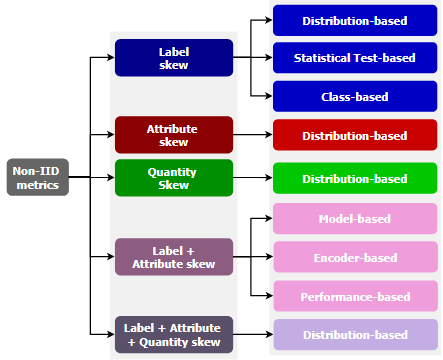
\includegraphics[width=\textwidth,height=0.7\textheight,keepaspectratio]{figures/jimenez_fig10.png}
    \vspace{0.15cm}

    {\fontsize{5.5pt}{7pt}\selectfont Jimenez et al. (2024), Figure 10: Taxonomy for non-IID metrics in Federated Learning.\\}
    \vspace{0.05cm}
    {\fontsize{8pt}{9.5pt}\selectfont Distribution-based metrics, like the Wasserstein distance, are required to measure attribute skew in continuous time-series energy data.}
    \vfill
\end{frame}

% ==========================================
% Topic 4: DynFed & Dynamic Quantization
% ==========================================

% Slide 9: Effects of heterogeneous quantization
\begin{frame}{DynFed \& Dynamic Quantization}
    \centering
    \vfill
    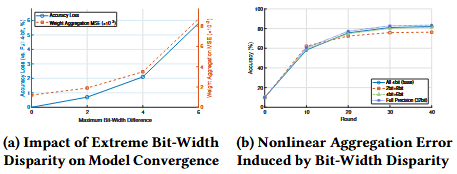
\includegraphics[width=\textwidth,height=0.7\textheight,keepaspectratio]{figures/dynfed_fig1.png}
    \vspace{0.15cm}

    {\fontsize{5.5pt}{7pt}\selectfont He et al. (2025 - DynFed), Figure 1: Effects of heterogeneous quantization bit-widths.\\}
    \vspace{0.05cm}
    {\fontsize{8pt}{9.5pt}\selectfont Bit-width disparities degrade standard FL aggregation, requiring a dynamic approach.}
    \vfill
\end{frame}

% Slide 10: Overview of training procedure
\begin{frame}{DynFed \& Dynamic Quantization}
    \centering
    \vfill
    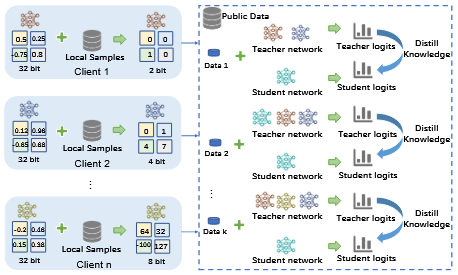
\includegraphics[width=\textwidth,height=0.7\textheight,keepaspectratio]{figures/dynfed_fig2.png}
    \vspace{0.15cm}

    {\fontsize{5.5pt}{7pt}\selectfont He et al. (2025 - DynFed), Figure 2: Overview of the training procedure proposed by DynFed.\\}
    \vspace{0.05cm}
    {\fontsize{8pt}{9.5pt}\selectfont The architecture relies on clients with varying bit-widths (e.g., 2-bit, 4-bit, 32-bit) extracting and distilling logits to a central server.}
    \vfill
\end{frame}

% Slide 11: Storage Cost and Total Time
\begin{frame}{DynFed \& Dynamic Quantization}
    \centering
    \vfill
    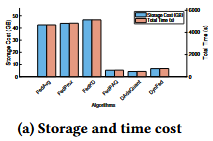
\includegraphics[width=\textwidth,height=0.7\textheight,keepaspectratio]{figures/dynfed_fig3a.png}
    \vspace{0.15cm}

    {\fontsize{5.5pt}{7pt}\selectfont He et al. (2025 - DynFed), Figure 3a: Storage Cost and Total Time comparison.\\}
    \vspace{0.05cm}
    {\fontsize{8pt}{9.5pt}\selectfont Dynamic quantization reduces communication overhead compared to uncompressed FedAvg or FedProx.}
    \vfill
\end{frame}

% Slide 12: Test Accuracy under heterogeneity
\begin{frame}{DynFed \& Dynamic Quantization}
    \centering
    \vfill
    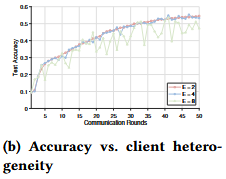
\includegraphics[width=\textwidth,height=0.7\textheight,keepaspectratio]{figures/dynfed_fig3b.png}
    \vspace{0.15cm}

    {\fontsize{5.5pt}{7pt}\selectfont He et al. (2025 - DynFed), Figure 3b: Test Accuracy under varying levels of client heterogeneity.\\}
    \vspace{0.05cm}
    {\fontsize{8pt}{9.5pt}\selectfont The algorithm maintains accuracy even when a large proportion of clients face resource limits.}
    \vfill
\end{frame}

% Slide 13: Adaptive quantization bit-width allocation
\begin{frame}{DynFed \& Dynamic Quantization}
    \centering
    \vfill
    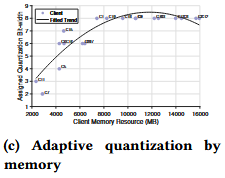
\includegraphics[width=\textwidth,height=0.7\textheight,keepaspectratio]{figures/dynfed_fig3c.png}
    \vspace{0.15cm}

    {\fontsize{5.5pt}{7pt}\selectfont He et al. (2025 - DynFed), Figure 3c: Adaptive quantization bit-width allocation mapped to client memory.\\}
    \vspace{0.05cm}
    {\fontsize{8pt}{9.5pt}\selectfont Assigned quantization bit-widths must positively correlate with a client's hardware capacity.}
    \vfill
\end{frame}

% Slide 14: Ablation study
\begin{frame}{DynFed \& Dynamic Quantization}
    \centering
    \vfill
    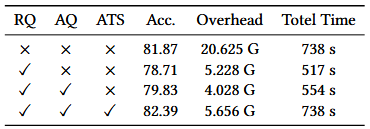
\includegraphics[width=\textwidth,height=0.7\textheight,keepaspectratio]{figures/dynfed_table2.png}
    \vspace{0.15cm}

    {\fontsize{5.5pt}{7pt}\selectfont He et al. (2025 - DynFed), Table 2: Ablation study of major components.\\}
    \vspace{0.05cm}
    {\fontsize{8pt}{9.5pt}\selectfont Combining Resource-Aware Quantization, Adaptive Loss Dynamics, and Active Teacher Selection yields peak accuracy.}
    \vfill
\end{frame}

% ==========================================
% Topic 5: Real-World Deployment
% ==========================================

% Slide 15: Architecture of energy management system
\begin{frame}{Real-World Deployment}
    \centering
    \vfill
    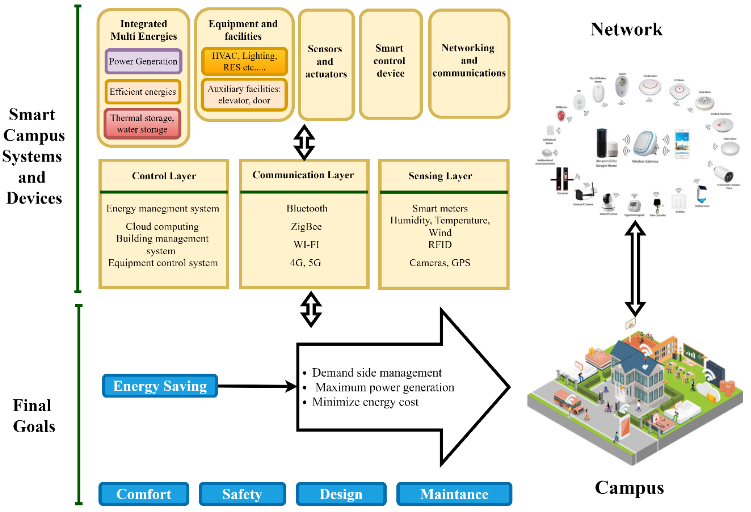
\includegraphics[width=\textwidth,height=0.7\textheight,keepaspectratio]{figures/manassra_fig9.png}
    \vspace{0.15cm}

    {\fontsize{5.5pt}{7pt}\selectfont Manassra and Işık (2025), Figure 9: Architecture of the AI-driven smart campus energy management system.\\}
    \vspace{0.05cm}
    {\fontsize{8pt}{9.5pt}\selectfont Real-world campus deployments may require a physical topology consisting of Sensing, Communication, and Control layers.}
    \vfill
\end{frame}

% Slide 16: Grafana dashboard
\begin{frame}{Real-World Deployment}
    \centering
    \vfill
    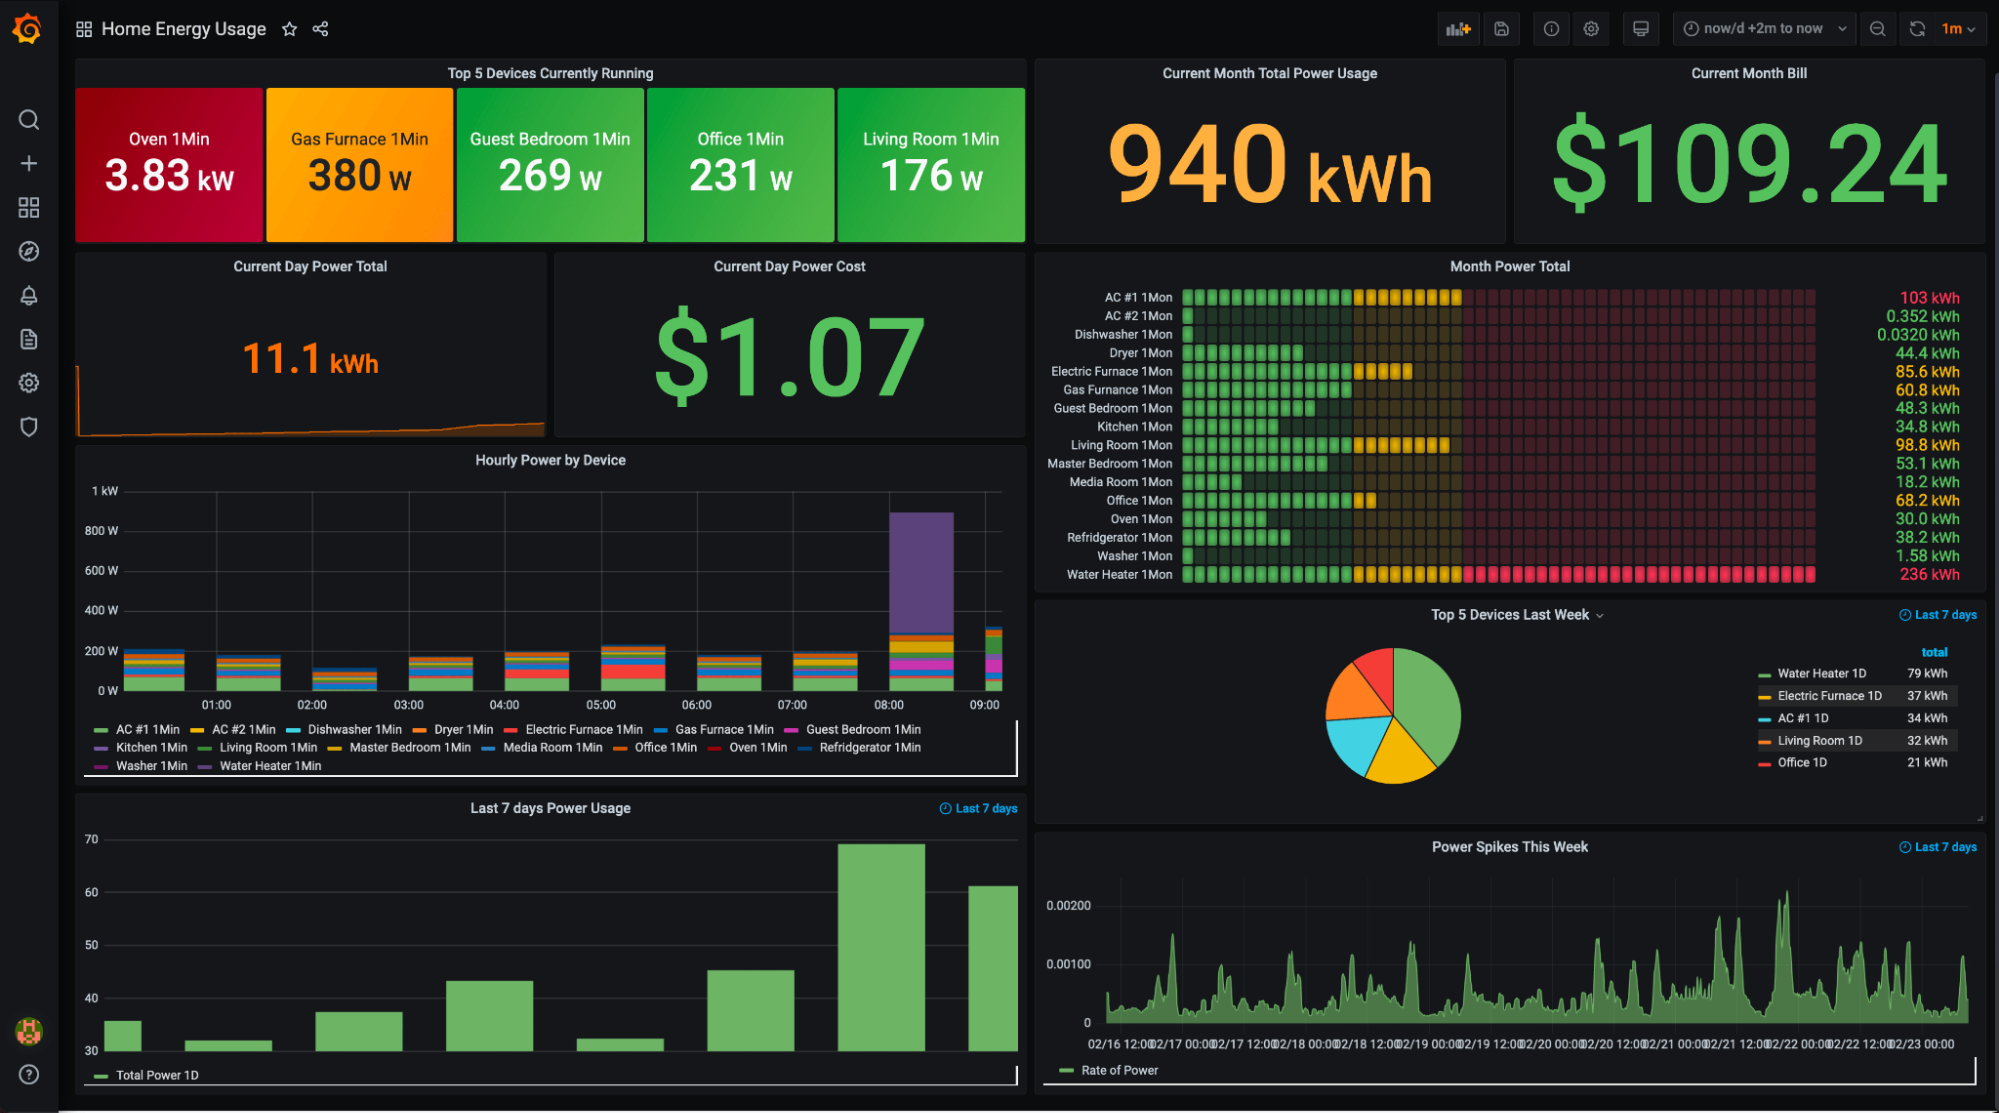
\includegraphics[width=\textwidth,height=0.7\textheight,keepaspectratio]{figures/grafana_dashboard.png}
    \vspace{0.15cm}

    {\fontsize{5.5pt}{7pt}\selectfont Grafana Smart Energy Dashboard.\\}
    \vspace{0.05cm}
    {\fontsize{8pt}{9.5pt}\selectfont A potential practical extension of my research.}
    \vfill
\end{frame}

% Slide 17: Commitments for This Week
\begin{frame}{Commitments for This Week}
    \begin{itemize}
        \item Continue studying and analyzing state-of-the-art adaptive quantization FL algorithms/protocols (e.g., DynFed, DAdaQuant).
        \item Continue investigating real-world pilot tests and operational implementations of FL for smart-city/campus energy management.
        \item Discuss with Sir Fritz the specifics of deploying IoT devices, sensors, etc., in DLSU and ALTDSI.
    \end{itemize}
\end{frame}

% Slide 18: Q&A / Standout Frame
\begin{frame}[standout]
    Thank You!
    \vspace{0.5cm}

    \begin{center}
        \large Questions \& Answers
    \end{center}
\end{frame}

\end{document}
